\chapter{Anwendungen von Predictive Analytics im öffentlichen Sektor}

Zum Schluss werden einige Anwendungen von Predictive Analytics im öffentlichen
Sektor vorgestellt. Es wurden Anwendungsfälle in den Bereichen öffentliche Verwaltung,
Gesundheit und Bildung betrachtet. Zudem wurden zwei Fallstudien erstellt, bei denen
zwei konkrete Anwendungen besonders ausführlich untersucht wurden.

% TODO
% 2 grundlegende Probleme
% - Datenschutz: Achtung Privatsphäre + Angst vor Missbrauch
% - Verzerrungen in Daten: insb. auch Big Data, Daten nicht repräsentativ,
%     Daten kulturabhängig

\section{Öffentliche Verwaltung}


\subsection{Open Data Portale}

Open Data Portale veröffentlichen Daten von Behörden, sodass prinzipiell jeder
sie nutzen kann. So existiert in den USA beispielsweise das Portal \glqq{Data.gov}\grqq{}\footnote{
URL für das US-Portal: \url{https://www.data.gov/}
}, das deutsche Pendant dazu heißt \glqq{GovData.de}\grqq{}\footnote{
URL für die deutsche Version: \url{https://www.govdata.de/} 
} (vgl. \cite{Borchers}). 

Grundsätzlich könnten die Daten auch für Predictive Analytics Zwecke genutzt werden.
Allerdings hat eine stichprobenartige Untersuchung ergeben, dass es sich bei vielen Daten
nicht mehr um \glqq{Rohdaten}\grqq{} handelt, sondern um eine aufbereitete Fassung, die sich
für die visuelle Präsentation eignet. Für Datenanalysen wären jedoch die Rohdaten besser geeignet.
Weiterhin scheinen manche Behörden im Vergleich zu anderen viele Daten an das Portal zu übergeben,
sodass die Auswahl dann unausgeglichen wirkt. Zudem gibt es die Kritik, dass viele relevante
Datensätze nicht veröffentlicht werden (vgl. \cite{Krempl}).

% TODO Daten (-> Heise) 
% Thapa_Parycek S. 46

Insgesamt ist aus der stichprobenartigen Untersuchung der Datensätze auf GovData.de nicht unmittelbar
hervorgegangen, wie die Daten für Predictive Analytics Anwendungen sinnvoll eingesetzt werden könnten. 

\subsection{Predictive Analytics in der Steuerverwaltung}

Die Anwendungen von Predictive Analytics in der Steuerverwaltung werden in einer
Studie des \emph{Forum on Tax Administration} (FTA) diskutiert\footnote{
Deutschland ist bei dieser Studie allerdings nicht dabei.
}. Der folgende Text beschreibt diese Anwendungsfälle.

\subsubsection{Audit Case Selection}

Steuerbehörden führen Kontrollen von Unternehmen und Personen durch, um Steuerbetrug
aufzudecken und zu verringern. Um verfügbare Ressourcen besser einzusetzen, werden mit Hilfe
von Predictive Analytics die Fälle für die Prüfung priorisiert, bei denen der größte Betrugsverdacht
besteht (Risikogruppen). Dieser Prozess wird als \emph{Audit Case Selection} bezeichnet und ist das hauptsächliche
Anwendungsgebiet von Predictive Analytics in der Steuerverwaltung (vgl. \cite{OECD}, S.~20).

Eine Besonderheit dabei ist die Analyse sozialer Netzwerke (\emph{Social Network Analysis}; \cite{OECD}, S.~21-22),
die zur Aufdeckung besonderer Formen von Einkommenssteuerbetrug eingesetzt wird. Die Analyse sozialer Netzwerke kann
Risikogruppen finden, die von Analysen auf individueller Ebene übersehen werden. Bei der Analyse werden die Beziehungen
zwischen Individuen erkennbar und können als visualisierte Netzwerke betrachtet werden. Die weitere Analyse dieser Netzwerke
kann durch Sachbearbeiter erfolgen oder mit Hilfe von regelbasierten oder statistischen Modellen durchgeführt werden.

\subsubsection{Payment Compliance}

Das Ziel der Payment Compliance ist es, ausstehende Zahlungen möglichst einzufordern oder das Problem gar nicht erst
entstehen zu lassen (vgl. \cite{OECD}, S.~24). Die typische Aufgabe von Predictive Analytics ist hierbei, die
Steuerzahler herauszufiltern, bei denen das größte Risiko besteht, dass sie ihre Zahlungsverpflichtungen nicht erfüllen werden. 
Eine weitere Anwendung, ist herauszufinden, wie am effektivsten mit dieser Gruppe kommuniziert werden kann (Prescriptive Analytics).

\subsubsection{Debt Management}

Beim traditionellen Debt Management werden Gruppen von Hochrisikoschuldnern identifiziert, um vorhandene Ressourcen auf sie zu
konzentrieren (vgl. \cite{OECD}, S.~26). Bei einer neueren Methode (\emph{Uplift Modelling}) werden Fälle selektiert, die
mit möglichst hoher Wahrscheinlichkeit auf eine Intervention seitens der Behörde reagieren werden. 

\subsubsection{Verbesserung der Serviceleistungen für Steuerzahler}

Text Mining (inklusive \emph{Sentiment Analysis}) kommt bei den Steuerbehörden zum Einsatz, um die Kommunikation mit den
Steuerzahlern zu verbessern (vgl. \cite{OECD}, S.~27). So werden beispielsweise ankommende E-Mails in Singapur mit Hilfe
von Text Mining bearbeitet, um die Art der Anfrage herauszufinden (vgl. \cite{OECD}, S.~27-28). In einem Fall konnte eine
Gruppe ähnlicher Anfragen identifiziert werden, nachdem eine Steuerrichtlinie verändert worden war. Die Behörde war dann in
der Lage frühzeitig zu reagieren und die Steuerzahler zusätzlich zu informieren. Text Mining hat in Singapur die manuelle
Bearbeitung von E-Mail Anfragen abgelöst. Dies ermöglicht eine objektivere Verarbeitung der Anfragen, da weniger Missverständnisse
entstehen. Zusätzlich wird die Arbeitszeit der Sachbearbeiter eingespart.

\subsubsection{Entscheidungsunterstützung}

Die meisten Datenanalysen bei den Steuerbehörden werden durchgeführt, um operative
Entscheidungen zu unterstützen (vgl. \cite{OECD}, S.~28). Allerdings exisitieren auch
Anwendungen, die strategische und politische Entscheidungen unterstützen. So werden
Analysen zur Abschätzung der Steuerlücke (\emph{tax gap analysis};vgl. \cite{OECD}, S.~28) durchgeführt.
Weiterhin wird versucht, den Einfluss von Änderungen in der Steuerpolitik vorherzusagen. Ein Beispiel
dafür, wenn auch streng genommen keine Predictive Analytics Anwendung, ist das ökonomische Modell, das
2012 von den chinesischen Behörden erstellt wurde, um die Effekte einer Steuerreform auf die Wirtschaft
und die soziale Wohlfahrt abzuschätzen (vgl. \cite{OECD}, S.~29). Der entsprechende Bericht der
Datenanalysten spielte eine wichtige Rolle in dem folgenden Reformprozess.

\subsubsection{Probleme mit Daten}

Der Bericht des FTA enthält auch eine Diskussion einiger Probleme, die im Zusammenhang mit Daten
festgestellt wurden.

So gibt es Bedenken, ob die gesammelten Daten, die anschließend für das Training der Modelle verwendet werden,
repräsentativ sind (vgl. \cite{OECD}, S.~51). Denn die verwendeten Daten stammen oft von stark verzerrten
Stichproben, wie beispielsweise alten Untersuchungsfällen. Somit wird nur ein kleiner Ausschnitt aus der
Gesamtpopulation zum Training der Modelle verwendet, was zu Selektionseffekten und schließlich zu Verzerrungen
im Modell führt. Um dieses Problem zu beheben, beziehen US-Steuerbehörden ihre Daten aus zufällig ausgewählten
Stichproben von Steuerprüfungen, um die Daten repräsentativer zu gestalten (vgl. \cite{OECD}, S.~52).

Weiterhin werden die Daten für Predictive Analytics Projekte eigentlich für operative Zwecke erhoben und
gespeichert (vgl. \cite{OECD}, S.~52). Aus diesem Grund ergeben sich verpasste Gelegenheiten, denn manche Daten, die nicht sinnvoll
für operative Zwecke sind, können nützlich für Datenanalysen sein. Zum Beispiel werden Beanstandungsgründe nach
einer Steuerprüfung typischerweise nicht gespeichert. Diese Information wäre jedoch hilfreich, um gesonderte Modelle
für verschiedene Beanstandungsgründe zu erstellen (vgl. \cite{OECD}, S.~52). 

\subsection{Predictive Policing}

Predictive Policing bezeichnet die Erstellung von Datenanalysen, um Verbrechen zu verhindern, Verbrechensfälle zu lösen
und wahrscheinliche Ziele für Polizeieinsätze zu identifizieren (vgl. \cite{Perry}, S.~1-2). Dabei können diese Methoden
in folgende vier Kategorien eingeteilt werden (vgl. \cite{Perry}, S.~8-9):

\begin{description}

\item[(1) Vorhersage von Verbrechen:] \hfill \\
Bei diesen Methoden sollen Plätze und Zeiträume identifiziert werden,
bei denen das Risiko für Verbrechen besonders hoch ist.

\item[(2) Vorhersage von Kriminellen:] \hfill \\
Hierbei sollen einzelne Personen identifiziert werden, die ein Risiko
tragen, in Zukunft Verbrechen zu begehen.

\item[(3) Vorhersage von Täterprofilen:] \hfill \\
Diese Methoden sollen Täterprofile generieren, die begangene Verbrechen
den wahrscheinlichen Tätern zuordnen.

\item[(4) Vorhersage der Opfer von Kriminalität:] \hfill \\
Hierbei sollen bestimmte Gruppen oder Einzelpersonen identifiziert werden,
bei denen ein erhöhtes Risiko besteht, Opfer von Verbrechen zu werden.

\end{description} 

\begin{figure}%[!hbt]
\centering
\caption{Predictive Policing Prozess}
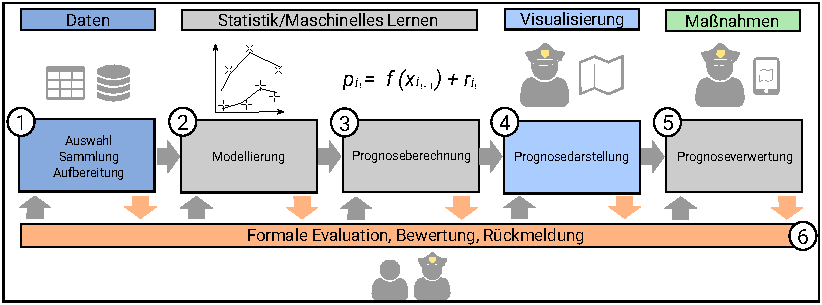
\includegraphics[scale=1.1]{Grafiken/Predictive_Policing_Ink.pdf} 
\label{pic:Predictive_Policing}
\end{figure}

In Deutschland werden bisher nur die Methoden von Punkt (1) verwendet, mit denen
Delikte wie Wohnungseinbrüche behandelt werden (vgl. \cite{Heuberger}).
Abbildung~\ref{pic:Predictive_Policing} zeigt hierbei das Vorgehen\footnote{
Das Original ist in \cite{Bode}, S.~2 zu finden.
}. Dies ist ähnlich zu den
allgemeinen Vorgehensmodellen aus Abschnitt~\xcom. Insbesondere die anwendungstypischen Details werden
im folgenden Text erläutert:

\begin{description}

\item[(1) Daten:] \hfill \\
Hierbei können polizeiliche und nicht-polizeiliche Daten kombiniert werden. Weiterhin
besteht die Notwendigkeit, die verschiedenen Daten korrekt zusammenzuführen, damit beispielsweise die räumliche
und zeitliche Konsistenz gewährleistet ist (vgl. \cite{Bode}, S.~2). Zudem werden bisher keine
personenbezogenen Daten verwendet (vgl. \cite{Bode}, S.~2 und \cite{Heuberger}) und die Daten konzentrieren
sich auf Wohnungseinbruchdiebstahl (vgl. \cite{Bode}, S.~2)

\item[(2) Modellierung:] \hfill \\
Für die Modellierung können die üblichen Algorithmen wie Regression, Entscheidungsbäume oder
neuronale Netze verwendet werden (vgl. \cite{Bode}, S.~2).

\item[(3) Prognoseberechnung:] \hfill \\
Das Ergebnis der Prognose ist eine Menge an Gebieten, die für den betrachteten Zeitraum
ein höheres Kriminalitätsrisiko aufweisen (vgl. \cite{Bode}, S.~2).

\item[(4) Prognosedarstellung:] \hfill \\
Neben der altmodischen Variante von Karten im Papierformat, existieren auch graphische
Visualisierungen mit Hilfe von Tablet-PCs oder Mobilfunkgeräten (vgl. \cite{Bode}, S.~3).

\item[(5) Prognoseverwertung:] \hfill \\
Die Prognosen werden durch operative Polizeieinheiten genutzt, die ihre Aktionen mit Hilfe
der Vorhersagen planen können (vgl. \cite{Bode}, S.~2).

\item[(6) Evaluation:] \hfill \\
Während das System arbeitet erfolgt auch immer wieder eine Bewertung der Leistung des Systems.
Die Evaluation beeinflusst die Schritte (1)-(5) (vgl. \cite{Bode}, S.~3).

\end{description}

\subsubsection{Bisheriges Fazit von Predictive Policing in Deutschland}

Bereits im RAND Bericht von 2013 wurde betont, dass Computer nicht von alleine die Probleme
lösen können. Es braucht viel Arbeit und Korrektureingriffe von Menschen (vgl. \cite{Perry}, S.~117-118). 
Dies ist sowohl auf datenanalytischer Ebene der Fall, als auch auf der sozialen Ebene, auf der
\glqq{Feldarbeit}\grqq{} notwendig ist, um das Wissen über die konkrete Kriminalitätsumgebung auf dem
neuesten Stand zu halten. 

Das Fazit von Predictive Policing in Deutschland ist bisher gemischt. Es gibt Berichte über hohe
Trefferquoten der Anwendungen. Diese sollten allerdings mit Skepsis beurteilt
werden, da bei der Berechnung der Trefferquoten mangels konkreter Regelungen Abweichungen
entstehen können (vgl. \cite{Bode}, S.~9).
Diese Unregelmäßigkeiten können in folgenden Bereichen entstehen (vgl. \cite{Bode}, S.~9-11):

\begin{description}
\item[Prognose-Delikt:] Welches Art des Delikts wurde konkret vorhergesagt?
\item[Prognose-Dauer:] Für welchen Zeitraum wurde die Prognose angefertigt?
\item[Prognose-Raum:] Zählen Treffer an Gebietsrändern?
\end{description}

Weiterhin kam ein Evaluationsbericht für die Anwendung des Predictive Policing Werkzeugs PRECOBS
zu dem Schluss, dass es schwer zu beurteilen ist, ob die Anwendung zu einer Verminderung von
Wohnungseinbrüchen geführt hat, und dass das Werkzeug wahrscheinlich nur zu einer moderaten Kriminalitätsminderung
beigetragen hat (vgl. \cite{Gerstner}, S.~85).  

\subsection{Wahlen und Politik}

Neben den in Abschnitt~\xcom erwähnten Text Mining Anwendungen zur Verbesserung der Serviceleistungen
von Behörden existieren noch weitere \glqq{experimentelle}\grqq{} Anwendungen. So konnte Matter durch
die Analyse teilstrukturierter Internetdokumente herausfinden, wie stark öffentliche Ämter in den USA
mit religiösen Personen besetzt sind (vgl. \cite{Matter}). Der \glqq{Bible Belt}\grqq{}\footnote{
Der \glqq{Bible Belt} ist eine besonders religiöse Region der USA, die sich über mehrere Bundesstaaten erstreckt.
} und der Mormonenstaat Utah waren deutlich als relgiös konservative Staaten erkennbar (vgl. \cite{Matter}, S.~1078).
Weiterhin konnten Falck et al. die weltanschauliche Nähe von Zeitungen zu politischen Parteien und einzelnen Politikern
darstellen, indem sie die Einstellungen der Zeitschriften zu den jeweiligen Personen und Parteien analysierten
(\emph{sentiment analysis}; vgl. \cite{Falck}, S.~4). Somit können mit Hilfe von Text Mining die weltanschaulichen Präferenzen
von Personen und Organisationen bestimmt werden. Allerdings ist der praktische Nutzen solcher Analysen (noch) nicht klar.
Personen, die sich mit Politik beschäftigen, können solche weltanschaulichen Differenzen mit Hilfe ihrer Erfahrung relativ
schnell einschätzen.

In den USA werden Datenanalysen bei Wahlkämpfen verwendet. So waren im Wahlkampfteam von
Hillary Clinton im Jahr 2016 mehr als 60 Mathematiker und Datenanalysten beschäftigt (vgl. \cite{Goldmacher}). 
Die Modelle, die sie anwenden, dienen unter anderem dazu, \glqq{Wackelkandidaten}\grqq{} unter Delegierten zu identifizieren,
um die verfügbaren Ressourcen an Wahlwerbung auf sie zu fokusieren (vgl. \cite{Goldmacher}). Allerdings hat Donald Trump bei der damaligen Wahl
fast nichts in Datenanalysen investiert (vgl. \cite{Goldmacher}) und trotzdem gewonnen.

Ein bekannteres (und umstritteneres) Beispiel für die Anwendung von Datenanalysen
für politische und wahlkampftaktische Ziele ist der Fall von Cambridge Analytica.

\subsubsection{Cambridge Analytica - Fallstudie}

\begin{figure}%[!hbt]
\centering
\caption{Nutzung von Facebook Likes zur Vorhersage von Nutzerattributen}
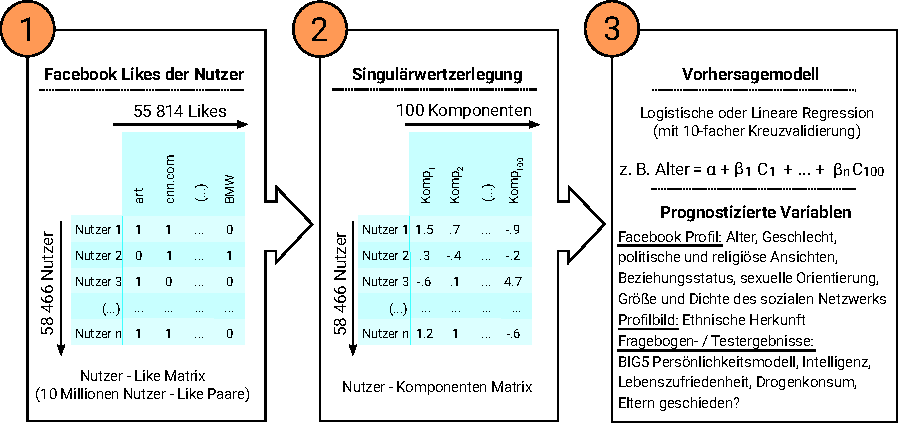
\includegraphics[scale=1.0]{Grafiken/Facebook_Likes_Ink.pdf} 
\label{pic:Like_Matrix}
\end{figure}

\section{Gesundheit}

Schon seit etwa 100 Jahren können statistische Methoden von Wissenschaftlern
genutzt werden, um Gefahren für die öffentliche Gesundheit zu untersuchen.

% TODO siehe Proctor

Diese Haltung war überraschend genug, um eine Nachfrage des Journalisten
auszulösen.


Das Thema Datenschutz bestimmt in Deutschland die Diskussion von Datenanalysen
im Gesundheitssektor.

% TODO
% Google Flu Trends (vorerst gescheitert)

% Kohortenstudien: nicht persönlich (s. Watson, Abschnitt Cohort treatment),
%   aber Sicherheitsbedenken bleiben (Anonymisierung nicht möglich, Sicherheits
%   risiken ...)

\subsection{Flint Trinkwasserskandal - Fallstudie}

\section{Bildung}
Abschließend sollen noch die Anwendungsmöglichkeiten von Predictive Analytics
im Bildungssektor kurz skizziert werden.

E$^2$

% Universitiy of Michigan E^2 Coach (Mattingly S. 242-243) 

Insgesamt scheint der Bildungssektor bisher am wenigsten von
Predictive Analytics Anwendungen profitiert zu haben.

% konkreteres Anwendungsbeispiel Decision Tree
